\chapter{Pixel-gebaseerde similariteitsmaten}

De similariteitsmaten die we in dit hoofdstuk beschouwen
meten de gelijkenis tussen twee afbeeldingen door hun beeldpunten met elkaar te vergelijken.
Deze beeldpunten worden ook \emph{picture elements} of kortweg \emph{pixels} genoemd. Vandaar
dat we zeggen dat deze maten \emph{pixel-gebaseerd} zijn.

\section{Grijswaardebeelden}

\subsection{Representatie}

Een \emph{binair beeld} is een beeld dat enkel witte en zwarte beeldpunten bevat. We kunnen een 
$n$-dimentionaal binair beeld dus modelleren als een scherpe verzameling $A$ in $\mathbb{R}^n$, met:
$$
\begin{array}{rcl}
x \in A & \iff & x \textrm{ is een wit punt in het beeld} \\
x \notin A & \iff & x \textrm{ is een zwart punt in het beeld}
\end{array}
$$ 
In de praktijk wordt een binair beeld echter voorgesteld als een rooster bestaande uit een
eindig aantal beeldpunten. Men kiest dus eerder $\mathbb{N}^2$ als universum.

Behalve wit en zwart, kan een \emph{grijswaardebeeld} ook grijstinten bevatten. Deze grijstinten
kunnen voorgesteld worden aan de hand van waarden uit het open eenheidsinterval $]0,1[$, waarbij
geldt: hoe groter de grijswaarde, hoe lichter de grijstint. Een $n$-dimensionaal grijswaardebeeld
kan dus gemodelleerd worden als een vaagverzameling $A$ in $\mathbb{R}^n$ bepaald door:
$$
\begin{array}{rcl}
A(x) = 1 & \iff & x \textrm{ is een wit punt in het beeld} \\
A(x) = 0 & \iff & x \textrm{ is een zwart punt in het beeld} \\
A(x) \in\ ]0,1[ & \iff & x \textrm{ is een beeldpunt met een grijstint}
\end{array}
$$
Ook bij grijswaardebeelden is het universum in de praktijk eerder $\mathbb{N}^2$.

\subsection{Similariteitsmaten}

Door de bovenstaande representatie te combineren met de vaagsimilariteitsmaten uit 
\ref{sectie:vaagsimilariteitsmaten}, bekomen we 23 similariteitsmaten voor grijswaardebeelden.
Hiermee kunnen we in onze praktische implementatie echter weinig aanvangen, vermits de
meeste afbeeldingen op internet kleurbeelden zijn. 


\section{Kleurbeelden}
\label{sectie:pixelgeb_kleurbeelden}

\subsection{Kleurruimten}

Een \emph{kleurmodel} is een abstract mathematisch model dat beschrijft hoe kleuren gerepresenteerd 
kunnen worden als $n$-tallen. RGB is het meest gebruikte kleurmodel. In dit model is elke kleur
een gewogen som van drie hoofdkleuren: rood, groen en blauw. De gewichten van deze som
worden gebruikt als componenten van het drietal dat de kleur voorstelt. Naast RGB zijn ook
HSV en L*a*b* populaire kleurmodellen \cite{phillips:beeldverwerking}.

De kleuren die men op basis van een bepaald model kan voorstellen vormen een \emph{kleurruimte}. 
In het geval van RGB is dit een driedimensionale ruimte. De kleuren in deze ruimte zijn afhankelijk
van de manier waarop men ``rood'', ``groen'' en ``blauw'' definieert. Veelgebruikte kleurruimtes 
op basis van het RGB model zijn sRGB en Adobe RGB.

Hoewel het strikt gezien niet correct is, gebruikt men de term ``kleurruimte'' vaak ook voor het
kleurmodel. Men heeft het dus vaak over \emph{de} RGB kleurruimte, terwijl er eigenlijk meerdere
kleurruimtes bestaan die gebaseerd zijn op RGB. 

\subsection{Representatie}

In een \emph{kleurbeeld} heeft elke pixel een bepaalde kleur. Deze kleur wordt beschreven met
behulp van een kleurmodel. Ze wordt bijgevolg voorgesteld als een $n$-tal uit
$\mathbb{R}^n$. Dergelijke $n$-tallen kunnen we normaliseren tot $n$-tallen uit $[0,1]^n$. 

We beperken ons tot het RGB model en we beschouwen de ordening $\leq_{RGB,lex}$, die
gebaseerd is op de lexicografische ordening $\leq_{lex}$ en op de ordening voor kleuren in het 
RGB model uit \cite{dewitte:vect_morph_ops}:
$$
\begin{array}{rcl}
c <_{RGB} c' & \iff & d(c,Bl) < d(c',Bl)\ \lor \\
			   &	  & \quad(d(c,Bl) = d(c',Bl) \land d(c,Wh) > d(c',Wh)) \\[5pt]
c >_{RGB} c' & \iff & d(c,Wh) < d(c',Wh)\ \lor \\
			   &	  & \quad(d(c,Wh) = d(c',Wh) \land d(c,Bl) > d(c',Bl)) \\[5pt]
c =_{RGB} c'   & \iff & (d(c,Bl) = d(c',Bl) \land d(c,Wh) = d(c',Wh)) \\[10pt]
c \leq_{lex} c' & \iff & r < r' \lor (r = r' \land g < g') \lor (r = r' \land g = g' \land b < b') \\[10pt]
c \leq_{RGB,lex} c' & \iff & c <_{RGB} c' \lor (c =_{RGB} c' \land c \leq_{lex} c')
\end{array}
$$
waarbij $Bl = (0,0,0)$, $Wh = (1,1,1)$ en $d$ de Euclidische afstand.
Men kan gemakkelijk verifi\"eren dat $([0,1]^3,\leq_{RGB,lex})$ een complete tralie is, met:
$$
\begin{array}{@{}c@{}}
\begin{array}{rcrcll}
\inf \{c,c'\} & = & \min \{c,c'\} & = & c & \textrm{als } c <_{RGB} c' \\
		  	& & & = & c' & \textrm{als } c >_{RGB} c' \\
		  	& & & = & c & \textrm{als } c =_{RGB} c' \textrm{ en } c \leq_{lex} c' \\
		  	& & & = & c' & \textrm{anders} \\[10pt]
\sup \{c,c'\} & = & \max \{c,c'\} & = & c' & \textrm{als } c <_{RGB} c' \\
		  	& & & = & c & \textrm{als } c >_{RGB} c' \\
		  	& & & = & c' & \textrm{als } c =_{RGB} c' \textrm{ en } c \leq_{lex} c' \\
		  	& & & = & c & \textrm{anders}
\end{array}
\end{array}
$$
We kunnen een $m$-dimensionaal RGB-kleurbeeld dus modelleren als een L-vaagverzameling in 
$\mathbb{R}^m$, waarbij $L=[0,1]^3$. Net zoals bij grijswaardebeelden, is 
het universum in de praktijk echter eerder $\mathbb{N}^2$.

\subsection{Similariteitsmaten}

De klassieke manier om kleurbeelden te vergelijken gaat als volgt. Men past een similariteitsmaat 
voor grijswaardebeelden toe op elk van de kleurcomponenten en voegt daarna de resultaten van de
verschillende componenten samen. In het geval van het RGB model beschouwt men een
kleurbeeld dus als een combinatie van drie grijswaardebeelden. 

Een andere mogelijkheid is dat men het beeld eerst omzet naar een grijswaardebeeld, om er 
vervolgens een similariteitsmaat voor grijswaardebeelden op toe te passen. Deze omzetting kan 
bijvoorbeeld aan de hand van de formule $y = 0.3 \cdot r + 0.59 \cdot g + 0.11 \cdot b$ gebeuren.

In \ref{sectie:vaagsimilariteitsmaten} hebben echter vermeld dat de beschouwde 
vaagsimilariteitsmaten uitbreidbaar zijn naar L-vaag\-ver\-za\-me\-ling\-en met
$L=[0,1]^3$. Daarvoor moeten we de bewerkingen waarvan deze maten gebruik maken veralgemenen van 
$[0,1]$ naar $[0,1]^3$. 
Voor de vaagsimilariteitsmaten $M_1$ tot $M_3$ betekent dit concreet dat we een zinvolle betekenis 
moeten geven aan $c - c'$ en $|c|$, voor alle $c(r,g,b),c'(r',g',b') \in [0,1]^3$. We gebruiken
hiervoor 
$$
c - c' = (r-r',g-g',b-b') \quad \textrm{ en } \quad |c| = \frac{1}{\sqrt{3}} \cdot \sqrt{r^2 + g^2 + b^2}.
$$
Om de overige vaagsimilariteitsmaten te veralgemenen, hebben we een uitbreiding van het
begrip sigma count nodig. Hiervoor gebruiken we
$$
|A|=\frac{1}{\sqrt{n}}\sum_{x \in X}\sqrt{(A_1(x))^2+(A_2(x))^2+\ldots+(A_n(x))^2}
$$
met $n=3$. Deze overige maten maken bovendien ook gebruik van de bewerkingen $co$ (complement), 
$\cap$ (doorsnede) en $\cup$ (unie). Doordat we 
$(\mathcal{N},\mathcal{C},\mathcal{D})=(N_s,T_M,S_M)$ gekozen hebben, moeten we
dus $1 - c$, $\max \{c,c'\}$ en $\min \{c,c'\}$ kunnen bepalen voor alle 
$c(r,g,b),c'(r',g',b') \in [0,1]^3$. Hiervoor kunnen we $1 - c = (1,1,1) - (r,g,b)$ en de
bovenstaande definities gebruiken.

We kunnen kleurbeelden dus ook vergelijken door de bovenstaande representatie 
te combineren met (een veralgemeende versie van) \'e\'en van de 
vaagsimilariteitsmaten uit \ref{sectie:vaagsimilariteitsmaten}. 
Deze tralie-gebaseerde aanpak lijkt ons de meest interessante van de drie, omdat
de kleur-informatie hierbij het best behouden blijft. De componenten van een kleur
in het RGB-model zijn namelijk sterk gecorreleerd, waardoor we informatie verliezen
als we ze elk afzonderlijk beschouwen. 


\section{Resolutie-onafhankelijk}
\label{sectie:res-onafh}

Men noemt het aantal pixels in een afbeelding de \emph{resolutie} van die afbeelding.
Een belangrijke beperking van de bovenstaande pixel-gebaseerde similariteitsmaten is dat we
ze enkel kunnen toepassen op beelden die dezelfde resolutie hebben. We kunnen dit oplossen
door similariteitsmaten te construeren op een manier die ge\"inspireerd is op de constructie
van de zogenaamde omgeving-gebaseerde similariteitsmaten in \cite{vanderweken:similariteitsmaten}. 

Deze constructie gaat als volgt. Stel dat we twee afbeeldingen $A$ en $B$ willen
vergelijken. We verdelen
de te vergelijken afbeeldingen eerst in twee partities, die respectievelijk bestaan uit
$n$ en $m$ beeldonderdelen. Hierbij zorgen we ervoor dat de onderdelen
van deze beide partities allemaal dezelfde resolutie hebben. We kunnen deze onderdelen bijgevolg 
opvatten als kleine afbeeldingen, die men onderling kan vergelijken met behulp van de reeds 
geziene pixel-gebaseerde similariteitsmaten.

Vervolgens bepalen we de gemiddelde kleur van elk beeldonderdeel. Deze kleur gebruiken we om
de collecties van beeldonderdelen voor te stellen als twee geordende lijsten, op basis
van de ordening $\leq_{RGB,lex}$. De elementen van de lijst die correspondeert met $A$ noemen 
we $A_i$, $i \in \{1,2,\ldots,n\}$, en die van de andere lijst $B_j$, $j \in \{1,2,\ldots,m\}$.

Figuur~\ref{fig:multires} illustreert de constructie van deze lijsten voor twee concrete
kleurbeelden. In deze figuur is de kleur van een beeldonderdeel gelijk aan de gemiddelde 
kleur van dat onderdeel.

Zodra we beschikken over de twee geordende lijsten, overlopen we de elementen van de 
lijst die correspondeert met $B$. Voor
elk element dat we tegenkomen, bepalen we de similariteit met $A_1$. Dit blijven we doen
tot we een similariteit vinden die kleiner is dan de vorige. We stoppen dus na $i$ iteraties 
indien $A_1$ en $B_i$ minder gelijkenis vertonen dan $A_1$ en $B_{i-1}$. Op dat moment voegen
we de similariteit tussen $A_1$ en $B_{i-1}$ toe aan de lijst van similariteiten $S$. Daarna
beginnen we bij $B_i$ en herhalen we deze procedure voor $A_2$. We voegen dus opnieuw de vorige
similariteit toe aan $S$ als deze groter is dan de huidige. Zo gaan we verder tot we bij
$B_m$ komen. Als we deze procedure $j$ keer kunnen herhalen, dan
is de similariteit tussen $A_j$ en $B_m$ dus de laatste die we berekenen. Deze similariteit
voegen we ook nog toe aan $S$. Tenslotte bepalen we de globale similarteit tussen $A$ en $B$ 
door het gemiddelde van de waarden uit $S$ te berekenen.

Tabel~\ref{tab:multires} geeft een overzicht van de 
verschillende similariteiten die berekend worden indien we de bovenstaande constructie
toepassen op de kleurbeelden uit figuur~\ref{fig:multires}. We hebben hierbij gebruik gemaakt 
van de vaagsimilariteitsmaat $M_3$ en de tralie-gebaseerde aanpak uit \ref{sectie:pixelgeb_kleurbeelden}.
De similariteiten die  
toegevoegd worden aan $S$ staan in het vet. Deze similariteiten 
worden in figuur~\ref{fig:multires} grafisch weergeven als verbindingen tussen de
geordende beeldonderdelen.

\begin{figure}[tbp]
\begin{center}
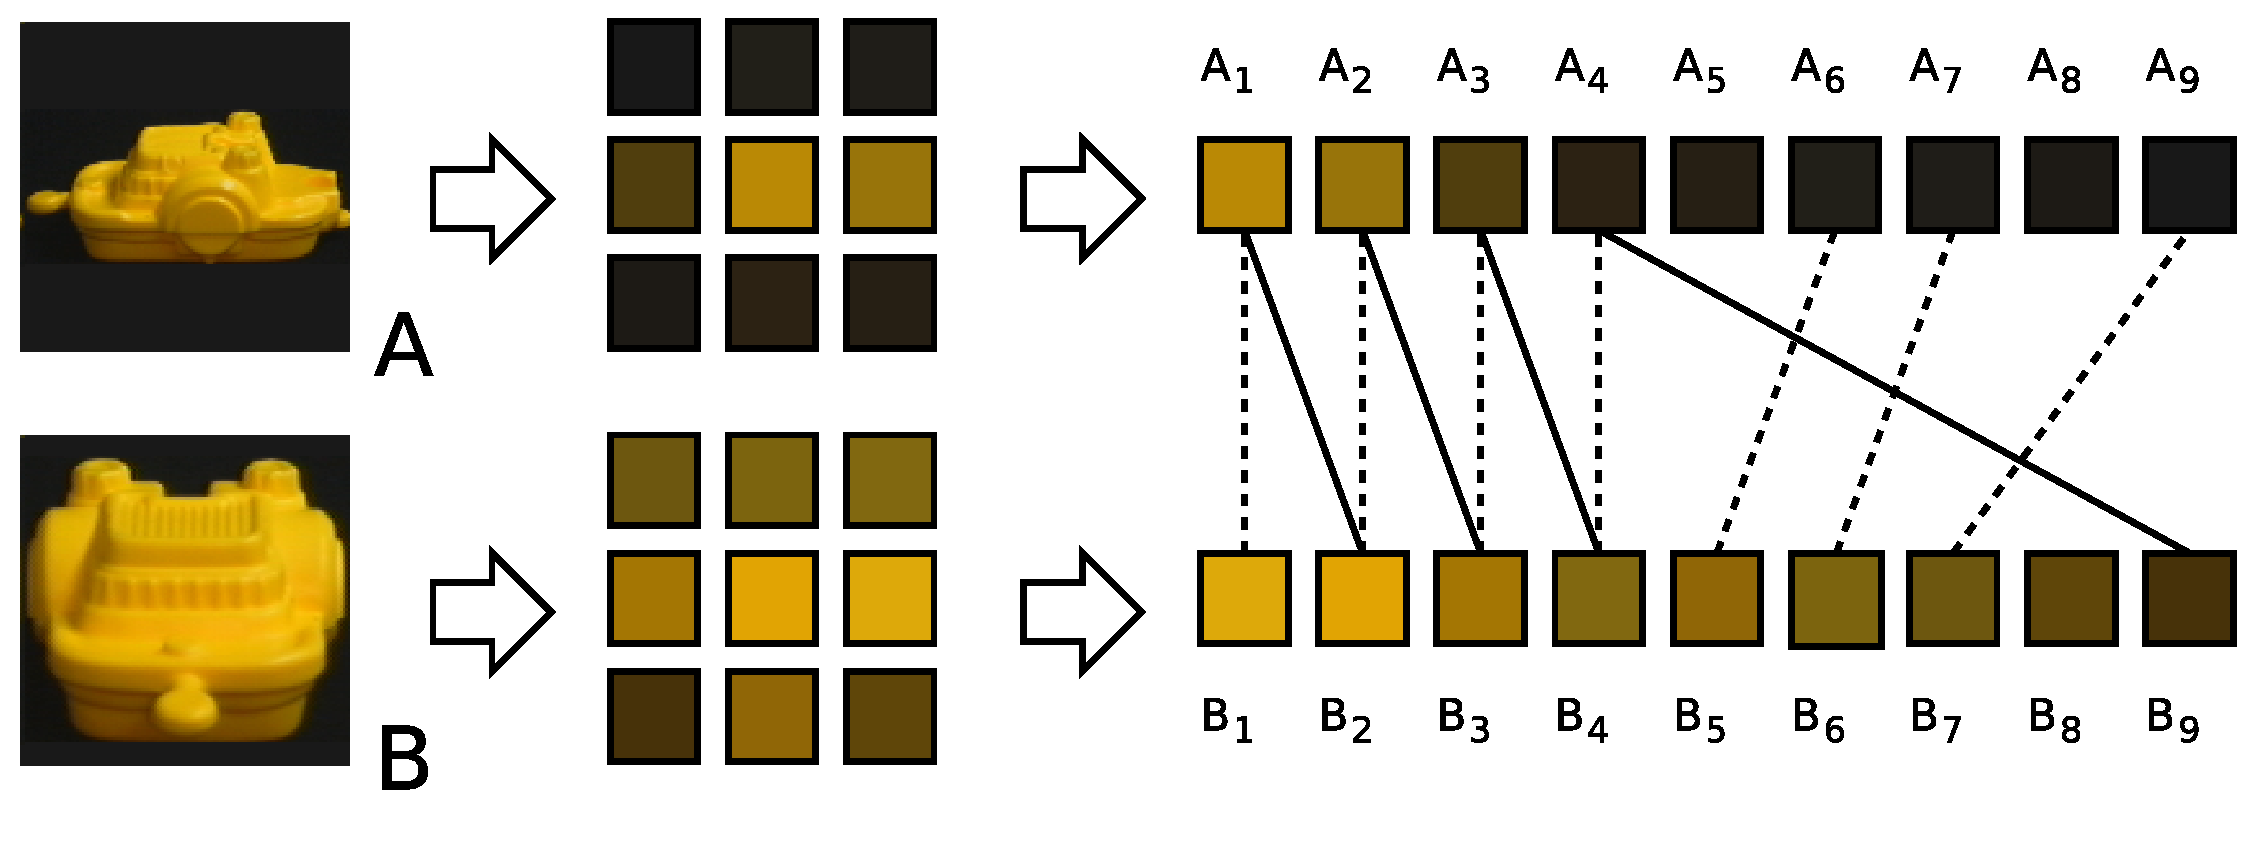
\includegraphics[width=\textwidth]{images/multires.eps}
\caption{\label{fig:multires}Constructie van een resolutie-onafhankelijke similariteitsmaat op basis van een pixel-gebaseerde maat.}
\end{center}
\end{figure}
\begin{table}
\begin{center}
\begin{tabular}{|c|ccccccccc|}
\hline
$\scriptstyle M_3(A_i,B_j)$	& $B_1$ & $B_2$ & $B_3$ & $B_4$ & $B_5$ & $B_6$ & $B_7$ & $B_8$ & $B_9$  \\
\hline
$A_1$ 	& $\mathbf{\scriptstyle 0.5198}$ & $\scriptstyle 0.4496$ & & & & & & & \\
$A_2$ 	& & $\mathbf{\scriptstyle 0.4691}$ & $\scriptstyle 0.3859$ & & & & & & \\
$A_3$ 	& & & $\scriptstyle 0.4133$ & $\mathbf{\scriptstyle 0.4404}$ & $\scriptstyle 0.3298$ & & & & \\
$A_4$ 	& & & & & $\scriptstyle 0.3277$ & $\mathbf{\scriptstyle 0.4330}$ & $\scriptstyle 0.3648$ & & \\
$A_5$ 	& & & & & & & $\mathbf{\scriptstyle 0.3849}$ & $\scriptstyle 0.3134$ & \\
$A_6$ 	& & & & & & & & $\mathbf{\scriptstyle 0.3438}$ & $\scriptstyle 0.3427$ \\
$A_7$ 	& & & & & & & & & $\mathbf{\scriptstyle 0.5066}$ \\
\hline
\end{tabular}
\caption{\label{tab:multires}De similariteiten die berekend worden in de constructie die ge\"illustreerd wordt door figuur~\ref{fig:multires}.}
\end{center}
\end{table}

De constructie van een resolutie-onafhankelijke similariteitsmaat, 
op basis van een pixel-gebaseerde maat, bestaat dus uit vier stappen:
\begin{enumerate}
\item Verdeel de te vergelijken afbeeldingen $A$ en $B$
in partities, zodanig dat alle beeldonderdelen dezelfde resolutie hebben.
\item Bepaal de gemiddelde kleur van elk beeldonderdeel. Gebruik deze kleur vervolgens
om de beide collecties van beeldonderdelen te ordenen met behulp van de ordening $\leq_{RGB,lex}$.
\item Overloop de beeldonderdelen van $B$ en bepaal telkens de similariteit met het eerste 
beeldonderdeel van $A$. Voeg de vorige similariteit toe aan de lijst van similariteiten $S$
indien ze groter is dan de huidige. Herhaal deze stap op dat moment voor de resterende
beeldonderdelen van $A$ en $B$. Het 
beeldonderdeel van $B$ dat aanleiding gaf tot de huidige similariteit maakt deel uit van
deze resterende beeldonderdelen.

Als het laatste beeldonderdeel van $B$ bereikt wordt, dan wordt de similariteit tussen dit
beeldonderdeel en het huidige beeldonderdeel van $A$ toegevoegd aan $S$. De overblijvende
beeldonderdelen van $A$ worden dan buiten beschouwing gelaten. 
\item Bepaal het gemiddelde van de similariteiten uit $S$. Deze waarde is de globale similariteit tussen
$A$ en $B$.
\end{enumerate}

Het resultaat $M$ van deze constructie, voor twee beelden $A$ en $B$, is echter niet noodzakelijk 
een symmetrische similariteitsmaat. Om dit probleem op te lossen, bepalen we zowel $M(A,B)$ als
$M(B,A)$ en gebruiken we het gemiddelde van deze waarden.


\section{Experimentele observaties}

\begin{figure}[tbp]
\begin{center}
\includegraphics[width=\textwidth]{plots/pixelgeb_gggrs_en_cputimes_filled.eps}
\caption{\label{fig:pixelgeb_gggrs_en_cputimes}De GGGR-waarde en de gebruikte rekentijd in ms voor elk van de resolutie-onafhankelijke pixel-gebaseerde similariteitsmaten.}
\end{center}
\end{figure}

In figuur~\ref{fig:pixelgeb_gggrs_en_cputimes} vergelijken we enkele pixel-gebaseerde similariteitsmaten.
Hoewel de afbeeldingen in onze testcollectie allemaal dezelfde resolutie hebben, zullen de
resoluties van de beelden die we in de praktijk gaan vergelijken vrijwel altijd verschillend zijn.
We beperken ons daarom tot resolutie-onafhankelijke similariteitsmaten. Deze maten construeren
we op basis van een pixel-gebaseerde maat, zoals besproken in \ref{sectie:res-onafh}. De 
beeldonderdelen die we gebruiken bestaan uit $8 \cdot 8 = 64$ pixels.

We beschouwen de drie bovenstaande manieren om de vaagsimilariteitsmaten toe te passen op een 
onderdeel van een kleurbeeld:
eerst omzetten naar een grijswaardebeeld, 
toepassen op de afzonderlijke kleurcomponenten en 
de tralie-gebaseerde aanpak.
De laatste manier in combinatie met $M_{3}$ levert de beste similariteitsmaat op. We vinden
voor deze similariteitsmaat de GGGR-waarde $0.16255411255411253$. Dit is echter nog steeds een
vrij hoge waarde. In figuur~\ref{fig:results_beste_pixelgeb}
zien we dan ook dat de resultaten van deze maat niet zo overtuigend zijn. Blijkbaar 
is de pixel-gebaseerde benadering niet de meest geschikte voor image retrieval. 

\begin{figure}[tbp]
\begin{center}
\begin{tabular}{m{11cm} | m{3cm} |}
\textbf{Eerste tien resultaten:} & \textbf{GGR:} \\
\vspace{4pt}
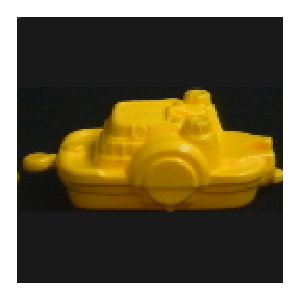
\includegraphics[width=1cm]{coil/beeld-12.eps}
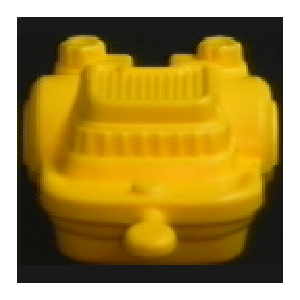
\includegraphics[width=1cm]{coil/beeld-14.eps}
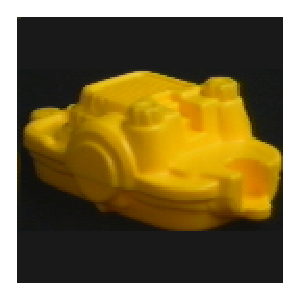
\includegraphics[width=1cm]{coil/beeld-16.eps}
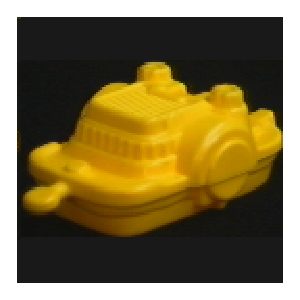
\includegraphics[width=1cm]{coil/beeld-15.eps}
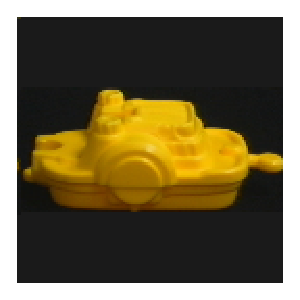
\includegraphics[width=1cm]{coil/beeld-13.eps}
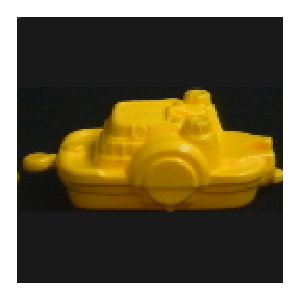
\includegraphics[width=1cm]{coil/beeld-12.eps}
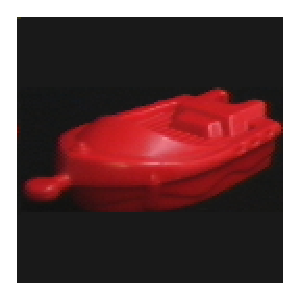
\includegraphics[width=1cm]{coil/beeld-21.eps}
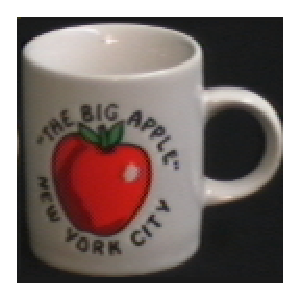
\includegraphics[width=1cm]{coil/beeld-36.eps}
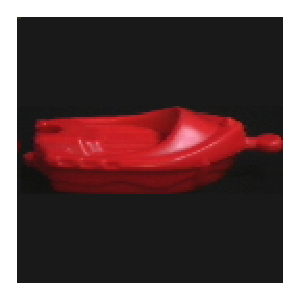
\includegraphics[width=1cm]{coil/beeld-19.eps}
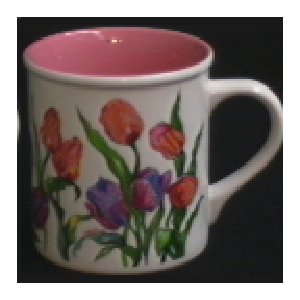
\includegraphics[width=1cm]{coil/beeld-6.eps}
& {\scriptsize 0.0}
\\
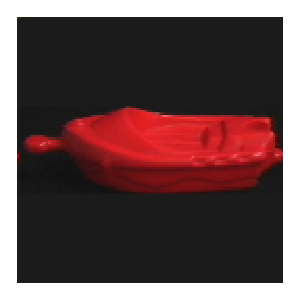
\includegraphics[width=1cm]{coil/beeld-18.eps}
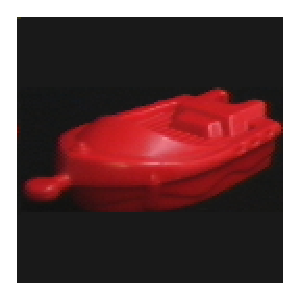
\includegraphics[width=1cm]{coil/beeld-21.eps}
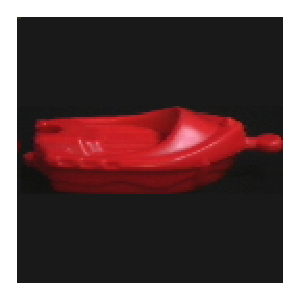
\includegraphics[width=1cm]{coil/beeld-19.eps}
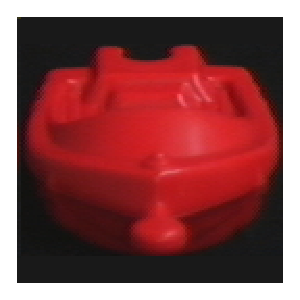
\includegraphics[width=1cm]{coil/beeld-20.eps}
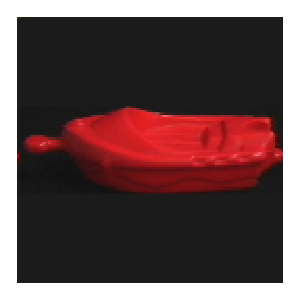
\includegraphics[width=1cm]{coil/beeld-18.eps}
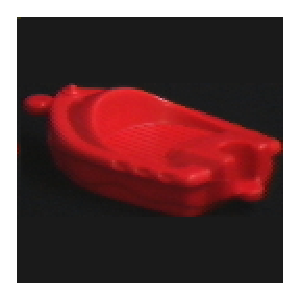
\includegraphics[width=1cm]{coil/beeld-22.eps}
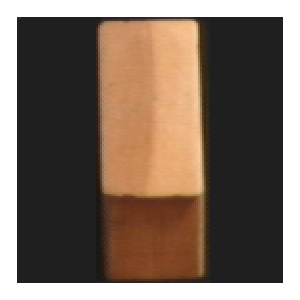
\includegraphics[width=1cm]{coil/beeld-44.eps}
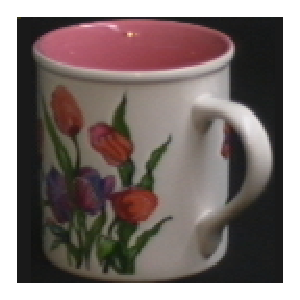
\includegraphics[width=1cm]{coil/beeld-10.eps}
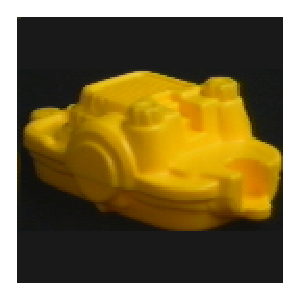
\includegraphics[width=1cm]{coil/beeld-16.eps}
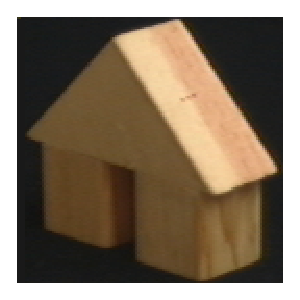
\includegraphics[width=1cm]{coil/beeld-46.eps}
& {\scriptsize 0.0}
\\
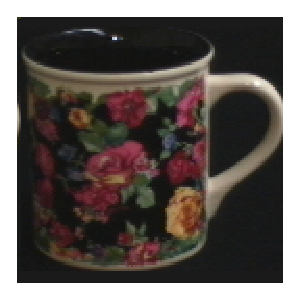
\includegraphics[width=1cm]{coil/beeld-60.eps}
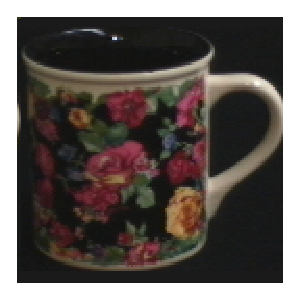
\includegraphics[width=1cm]{coil/beeld-60.eps}
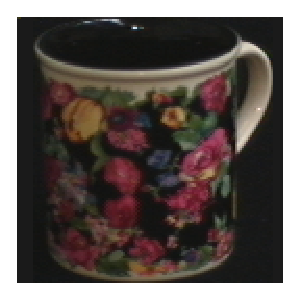
\includegraphics[width=1cm]{coil/beeld-63.eps}
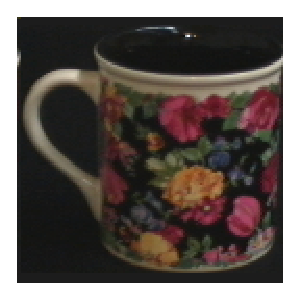
\includegraphics[width=1cm]{coil/beeld-61.eps}
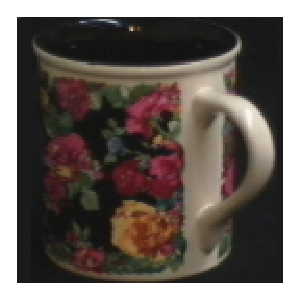
\includegraphics[width=1cm]{coil/beeld-64.eps}
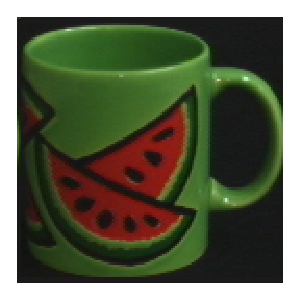
\includegraphics[width=1cm]{coil/beeld-30.eps}
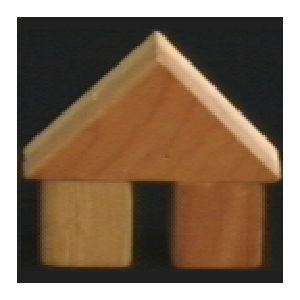
\includegraphics[width=1cm]{coil/beeld-43.eps}
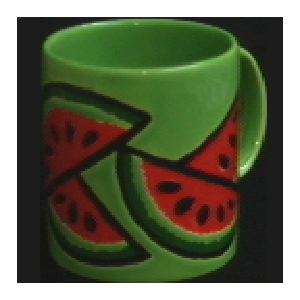
\includegraphics[width=1cm]{coil/beeld-33.eps}
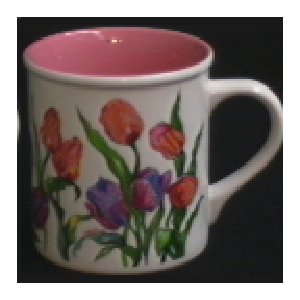
\includegraphics[width=1cm]{coil/beeld-6.eps}
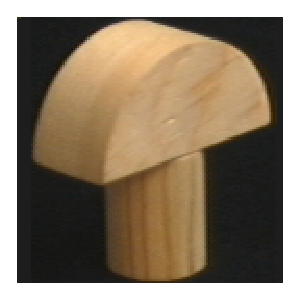
\includegraphics[width=1cm]{coil/beeld-3.eps}
& {\scriptsize 0.02619047619047619}
\\
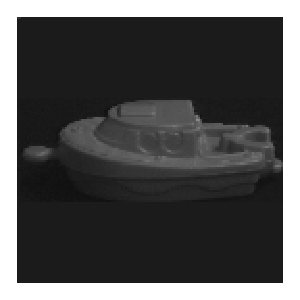
\includegraphics[width=1cm]{coil/beeld-24.eps}
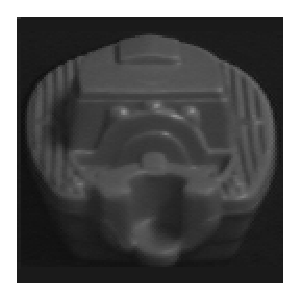
\includegraphics[width=1cm]{coil/beeld-26.eps}
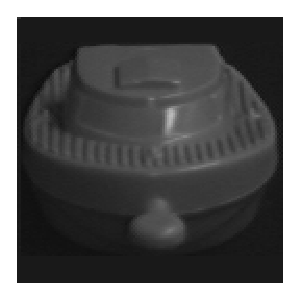
\includegraphics[width=1cm]{coil/beeld-28.eps}
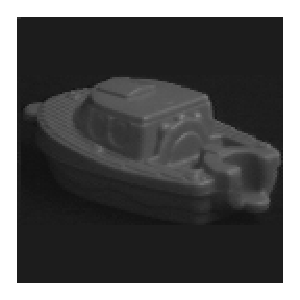
\includegraphics[width=1cm]{coil/beeld-25.eps}
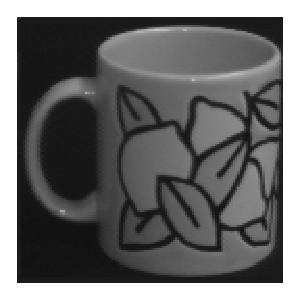
\includegraphics[width=1cm]{coil/beeld-49.eps}
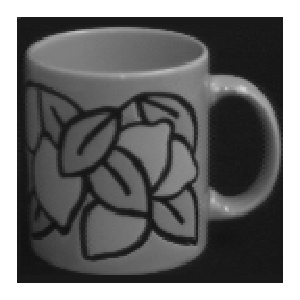
\includegraphics[width=1cm]{coil/beeld-48.eps}
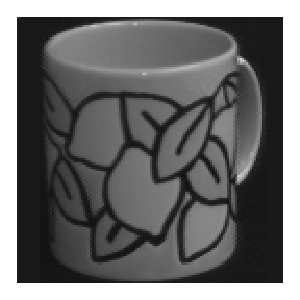
\includegraphics[width=1cm]{coil/beeld-51.eps}
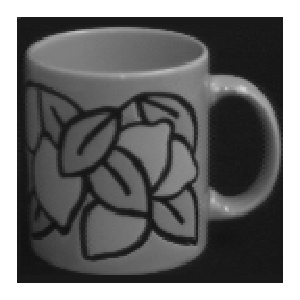
\includegraphics[width=1cm]{coil/beeld-48.eps}
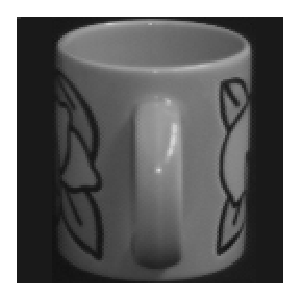
\includegraphics[width=1cm]{coil/beeld-50.eps}
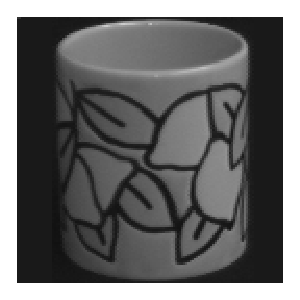
\includegraphics[width=1cm]{coil/beeld-52.eps}
& {\scriptsize 0.02857142857142857}
\\
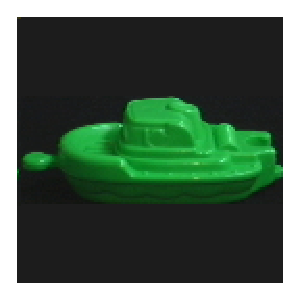
\includegraphics[width=1cm]{coil/beeld-54.eps}
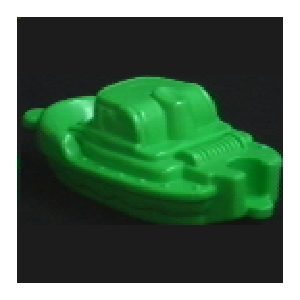
\includegraphics[width=1cm]{coil/beeld-58.eps}
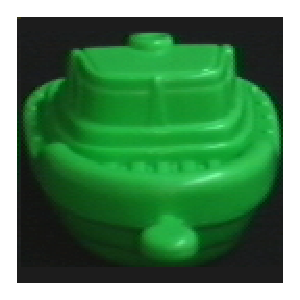
\includegraphics[width=1cm]{coil/beeld-56.eps}
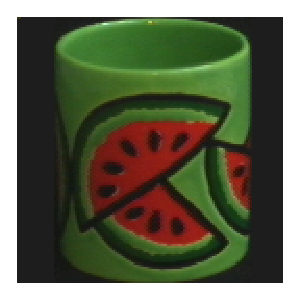
\includegraphics[width=1cm]{coil/beeld-32.eps}
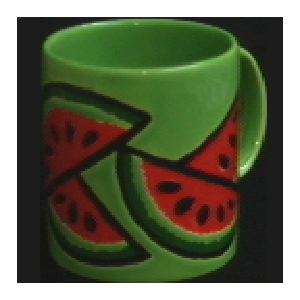
\includegraphics[width=1cm]{coil/beeld-33.eps}
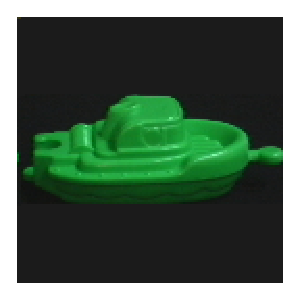
\includegraphics[width=1cm]{coil/beeld-55.eps}
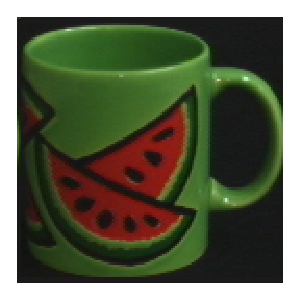
\includegraphics[width=1cm]{coil/beeld-30.eps}
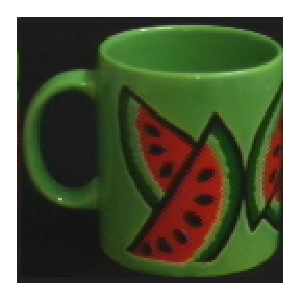
\includegraphics[width=1cm]{coil/beeld-31.eps}
\includegraphics[width=1cm]{coil/beeld-1.eps}
\includegraphics[width=1cm]{coil/beeld-30.eps}
& {\scriptsize 0.04523809523809524}
\\
\includegraphics[width=1cm]{coil/beeld-30.eps}
\includegraphics[width=1cm]{coil/beeld-33.eps}
\includegraphics[width=1cm]{coil/beeld-31.eps}
\includegraphics[width=1cm]{coil/beeld-32.eps}
\includegraphics[width=1cm]{coil/beeld-63.eps}
\includegraphics[width=1cm]{coil/beeld-57.eps}
\includegraphics[width=1cm]{coil/beeld-60.eps}
\includegraphics[width=1cm]{coil/beeld-3.eps}
\includegraphics[width=1cm]{coil/beeld-60.eps}
\includegraphics[width=1cm]{coil/beeld-1.eps}
& {\scriptsize 0.047619047619047616}
\\
\includegraphics[width=1cm]{coil/beeld-6.eps}
\includegraphics[width=1cm]{coil/beeld-9.eps}
\includegraphics[width=1cm]{coil/beeld-39.eps}
\includegraphics[width=1cm]{coil/beeld-7.eps}
\includegraphics[width=1cm]{coil/beeld-6.eps}
\includegraphics[width=1cm]{coil/beeld-64.eps}
\includegraphics[width=1cm]{coil/beeld-43.eps}
\includegraphics[width=1cm]{coil/beeld-3.eps}
\includegraphics[width=1cm]{coil/beeld-37.eps}
\includegraphics[width=1cm]{coil/beeld-60.eps}
& {\scriptsize 0.05238095238095238}
\\
\includegraphics[width=1cm]{coil/beeld-48.eps}
\includegraphics[width=1cm]{coil/beeld-24.eps}
\includegraphics[width=1cm]{coil/beeld-27.eps}
\includegraphics[width=1cm]{coil/beeld-25.eps}
\includegraphics[width=1cm]{coil/beeld-24.eps}
\includegraphics[width=1cm]{coil/beeld-49.eps}
\includegraphics[width=1cm]{coil/beeld-50.eps}
\includegraphics[width=1cm]{coil/beeld-28.eps}
\includegraphics[width=1cm]{coil/beeld-26.eps}
\includegraphics[width=1cm]{coil/beeld-51.eps}
& {\scriptsize 0.06190476190476191}
\\
\includegraphics[width=1cm]{coil/beeld-36.eps}
\includegraphics[width=1cm]{coil/beeld-3.eps}
\includegraphics[width=1cm]{coil/beeld-37.eps}
\includegraphics[width=1cm]{coil/beeld-6.eps}
\includegraphics[width=1cm]{coil/beeld-36.eps}
\includegraphics[width=1cm]{coil/beeld-7.eps}
\includegraphics[width=1cm]{coil/beeld-0.eps}
\includegraphics[width=1cm]{coil/beeld-9.eps}
\includegraphics[width=1cm]{coil/beeld-8.eps}
\includegraphics[width=1cm]{coil/beeld-6.eps}
& {\scriptsize 0.1261904761904762}
\\
\includegraphics[width=1cm]{coil/beeld-42.eps}
\includegraphics[width=1cm]{coil/beeld-0.eps}
\includegraphics[width=1cm]{coil/beeld-3.eps}
\includegraphics[width=1cm]{coil/beeld-42.eps}
\includegraphics[width=1cm]{coil/beeld-45.eps}
\includegraphics[width=1cm]{coil/beeld-1.eps}
\includegraphics[width=1cm]{coil/beeld-37.eps}
\includegraphics[width=1cm]{coil/beeld-33.eps}
\includegraphics[width=1cm]{coil/beeld-36.eps}
\includegraphics[width=1cm]{coil/beeld-0.eps}
& {\scriptsize 0.2642857142857143}
\\
\includegraphics[width=1cm]{coil/beeld-0.eps}
\includegraphics[width=1cm]{coil/beeld-42.eps}
\includegraphics[width=1cm]{coil/beeld-45.eps}
\includegraphics[width=1cm]{coil/beeld-39.eps}
\includegraphics[width=1cm]{coil/beeld-3.eps}
\includegraphics[width=1cm]{coil/beeld-43.eps}
\includegraphics[width=1cm]{coil/beeld-37.eps}
\includegraphics[width=1cm]{coil/beeld-64.eps}
\includegraphics[width=1cm]{coil/beeld-1.eps}
\includegraphics[width=1cm]{coil/beeld-0.eps}
& {\scriptsize 0.2714285714285714}
\end{tabular}
\caption{\label{fig:results_beste_pixelgeb}De GGR-waarde en de eerste tien resultaten voor elke voorbeeld-afbeelding bij de beste resolutie-onafhankelijke pixel-gebaseerde similariteitsmaat.}
\end{center}
\end{figure}

Op het vlak van rekentijd zijn de similariteitsmaten op basis van de eerste en de laatste manier
aan elkaar gewaagd. Bij het toepassen van een similariteitsmaat voor grijswaardebeelden op de 
afzonderlijke kleurcomponenten, hebben we echter aanzienlijk meer rekentijd nodig. Dit is niet
verwonderlijk, vermits er dan ook driemaal zoveel werk moet verricht worden.
